% !TeX spellcheck = en_US
\section{Problem 11}
Convolutional Neural Networks (CNNs) have revolutionized in the field of image processing and computer vision and are widely utilized.\\

In this exercise we are considering a $6 x 6$ image I, where each entry represents the intensity of a pixel.The values are typically normalized , and the CNN would perform operations on this matrix to learn features and perform tasks like classification, detection, or segmentation. We will apply various layers and filters, so that we can extract higher-level features.\\


\begin{equation}
	I = \begin{bmatrix}
		20 & 35 & 35 & 35 & 35 & 20 \\
		29 & 46 & 44 & 42 & 42 & 27 \\
		16 & 25 & 21 & 19 & 19 & 12 \\
		66 & 120 & 116 & 154 & 114 & 62 \\
		74 & 216 & 174 & 252 & 172 & 112 \\
		70 & 210 & 170 & 250 & 170 & 110 \\
	\end{bmatrix}
	\label{tab:input_image}
\end{equation}
\vspace{2mm}

Given the input matrix we can understand that it represents a grayscale image. In a grayscale image, each pixel is represented by a single intensity value, typically on a scale $\left[0, 255\right]$. The 2D input array contains such intensity values for each pixel in the image.

\subsection{Question A}
The output of a convolution layer is a new matrix that's the result of the convolution operation. The convolution operation involves sliding the kernel over the input matrix, with a given stride $\left(1,1\right)$, and for each position, computing the sum of elementwise multiplications. \\

The use of a stride in a convolutional layer is important, because it determines how much the filter or kernel moves across the input matrix. In our case, a stride of $\left(1,1\right)$ means that the kernel moves one step at a time horizontally and vertically. This will result in an output matrix that is smaller than the input matrix by one less than the kernel size in each dimension. So, in our case the output will be a $4 x 4$. Also,the output's matrix size is smaller than the original because of the "valid" mode on our code. The "valid" mode means that the convolution product is only given for points where the kernels overlap completely with the input array. It doesn't add any padding to the input image.\\

In addition, the kernel we have defined is a $3 x 3$ matrix with a zero in the center. This means that the convolution operation will sum up the values of the eight surrounding pixels and ignore the center pixel for each position in the input image.\\

So, in conclusion, with a
\begin{itemize}
	\item $stride = \left(1,1\right)$ and 
	\item $	kernel = \begin{bmatrix}
		1 & 1 & 1  \\
		1 & 0 & 1  \\
		1 & 1 & 1  \\
	\end{bmatrix}$
\end{itemize}

The result of the convolution is a $ 4 x 4$ matrix\\

\begin{equation}
	result = \begin{bmatrix}
		225 & 258 & 250 & 209  \\
		458 & 566 & 552 & 472  \\
		708 & 981 & 887 & 802  \\
		1000 & 1488 & 1320 &1224 \\
	\end{bmatrix}
\end{equation}
\vspace{6mm}

The resulting matrix, represents the features in the input image that the kernel was able to detect. In this case, the kernel seems to act like a filter that emphasizes the surrounding context of each pixel. The exact interpretation would depend on the specific values in the input image and the kernel. 

\begin{figure}[h]
	\centering
	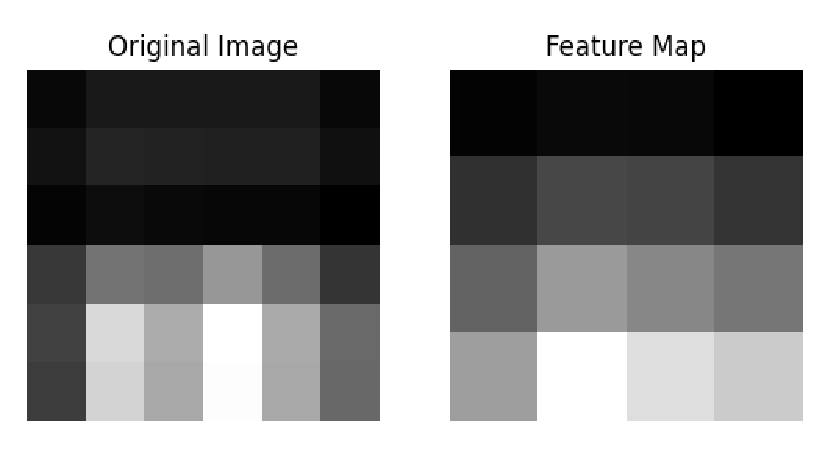
\includegraphics[width=.7\textwidth]{../Problem 11/conv_result.pdf}
	\caption{The Original Image and the Image after the convolution}
\end{figure}
\vspace{3mm}
\subsection{Question B}
Now, using the output of the convolution of the input image we are going to apply a max pooling layer with the following properties: 
\begin{itemize}
	\item $stride = \left(2,2\right)$ and 
	\item $	window\ \ shape = \left(2, 2\right)$
\end{itemize}
In general, a max pooling layer performs a downsampling operation along the spatial dimensions, width and height, of the input data. The main goal is to reduce the dimensionality of the input, which helps to control overfitting and reduces computational complexity for subsequent layers.\\
In our exercise, the size of the input matrix is reduced from $ 4 x 4 \rightarrow 2 x 2$.\\
 
The max pooling operation works by defining a spatial neighborhood, in our case a $ 2 x 2\ \ window$ and taking the maximum element from the rectified feature map within the window. This window is slid over the input data with a certain stride to produce a new matrix where each element is the maximum of a neighborhood from the input. This process effectively reduces the spatial dimensions of the feature map.\\

The result of the max pooling layer is a $2 x 2$ matrix of the same image
\begin{equation}
	max\_pooling = \begin{bmatrix}
		566 & 552   \\
		1488 & 1320 &  \\
	\end{bmatrix}
\end{equation}
\\
We can conclude that the max pooling operation only reduces the size of the feature map while preserving the most important and prominent features. It gives a more abstract and compressed representation of the input image.
\vspace{3mm}

\subsection{Question C}
As we have seen in the previous questions, the use of kernels, also known as filters, is a fundamental tool for image processing. They are essential for the efficient extraction of different features, the reduction of the number of parameters and optimal processing. In this exercise, we will emphasize the importance of kernels for extracting different features from the same input image.\\

So, for the input image (Matrix~\ref{tab:input_image}) we have the following results:
\begin{itemize}
	\item \underline{Filter $F1$}\\
	
	\begin{equation}
		F1 = \begin{bmatrix}
			-10 & -10 & -10   \\
			  5 &  5 &  5   \\
			-10 & -10 & -10   \\
		\end{bmatrix}
	\end{equation}
	\vspace{2mm}
	
	We can conclude that this filter is a type of edge detection filter, specifically designed to detect edges running horizontally in an image. \\
	In more detail, the negative values on the top and bottom rows will respond strongly to intensity changes in those directions, while the positive values in the middle row will respond to the opposite. Areas with strong horizontal edges will result in high absolute values in the convolved feature map. This means that this filter will highlight areas of the image where there is a strong intensity change from dark to light or light to dark in a horizontal direction, effectively detecting horizontal edges. To be precise, the positive values in the middle row of the kernel will align with the lighter part of a horizontal edge, while the negative values will align with the darker part.\\
	
	After applying the kernel $F1$ to our input image I, we obtain the following matrix:

	\begin{equation}
		I\_F1 = \begin{bmatrix}
			-925 & -1040 & -1000 & -845 \\
			 -3900 & -4895 & -4825 & -4160  \\
			-3750 & -5120 &-4650 & -4210   \\
			-5200 & -6990 & -6750 & -5920 \\
			\end{bmatrix}
	\end{equation}
	\vspace{2mm}
	
	As we can observe, the size of the matrix is reduced, due to the "valid" mode in the convolution operation on our code, as it only computes the convolution where the kernel fits entirely within the image boundaries.\\
	
	The values in this feature map represent the strength and location of horizontal edges detected in the input image. High absolute values, whether positive or negative, indicate strong edges, while values close to zero indicate regions with little or no horizontal edge presence.\\
	In this case, the large negative values indicate strong horizontal edges where there is a transition from light to dark pixels. This is consistent with the design of the kernel, which is tailored to detect such features in the image.
	
	
	To understand the topic, i will provide a graphical explanation.
	\begin{figure}[H]
		\centering
		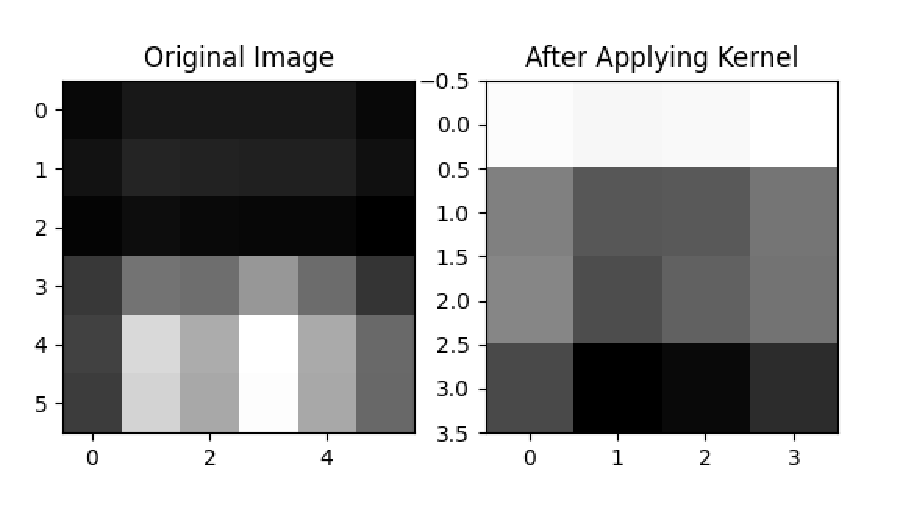
\includegraphics[width=.7\textwidth]{../Problem 11/kernel_F1.pdf}
		\caption{Before and After of the input image}
		\label{fig:kernel1}
	\end{figure}
	\vspace{3mm}
	
	\item \underline{Filter $F2$}\\
	
	\begin{equation}
		F2 = \begin{bmatrix}
			2 & 2 & 2   \\
			2 & -12 & 2   \\
			2 & 2 & 2   \\
		\end{bmatrix}
	\end{equation}
	\vspace{2mm}
	
	The filter $F2$ is a $3 x 3$ matrix with a negative value in the center and positive values surrounding it. This type of kernel is often used for edge detection, most likely to highlight the edges of objects in the image.\\
	
	This configuration indicates that the kernel is likely designed to detect points in the image where there is a central pixel that is significantly different from its surrounding pixels. Exemplifying, when this kernel is convoluted with an image, it computes a difference between the center pixel and its neighbors. If the image has a region where pixel intensity changes rapidly, the convolution operation will yield a high absolute value. In contrast, in regions of the image where pixel intensity changes slowly, the convolution operation will yield values close to zero.\\
	
	To have a better understanding, we will apply this kernel to our image I.\\
	After applying the kernel $F2$ to our image, the result is:
	
		\begin{equation}
		I\_F2 = \begin{bmatrix}
			-102 & -12 &  -4 & -86 \\
			 616  & 880 &  876 &  716  \\
			-24 & 570 & -74 & 236   \\
			-592 & 888 & -384 & 384 \\
		\end{bmatrix}
	\end{equation}
	\vspace{2mm}
	
	That being said, the positive and negative values in the feature map correspond to areas where this contrast is detected. Particularly, positive values indicate regions where the central pixel is much darker than its surroundings and negative values indicate regions where the central pixel is not significally different from its surroundings as in regions with higher positive values.\\
	
	We can figure it out by providing also this figure:
	\begin{figure}[H]
		\centering
		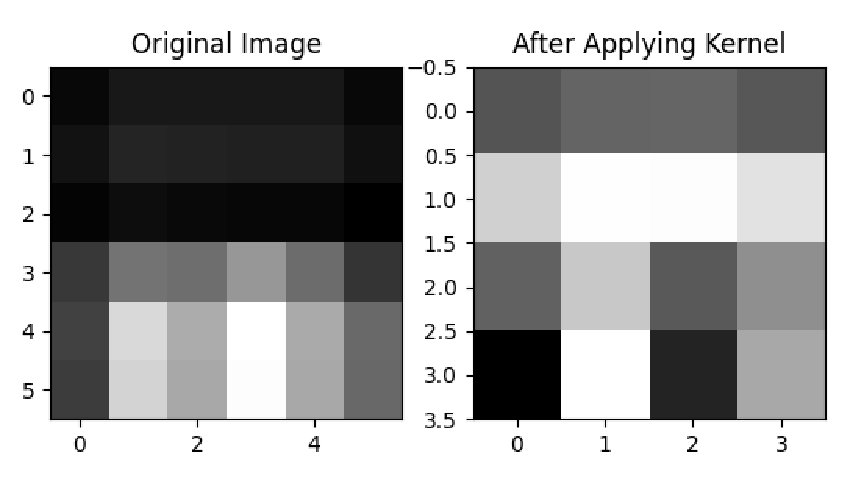
\includegraphics[width=.7\textwidth]{../Problem 11/kernel_F2.pdf}
		\caption{Before and After of the input image}
		\label{fig:kernel2}
	\end{figure}
	\vspace{3mm}
	
	The visualization in the image seems to reflect the application of such a kernel, because areas of the original image that had a central pixel with lower intensity compared to the neighbors would stand out as brighter spots in the resulting image.\\
	
	To sum up, this kind of kernel is useful for detecting features such as sharp edges, corners, or small isolated features where there is a notable contrast between a central point and its neighboring pixels. The high values (both positive and negative) in the feature map highlight these contrasting areas in the image.
	\vspace{3mm}
	
	\item \underline{Filter $F3$}\\
	
	\begin{equation}
		F3 = \begin{bmatrix}
			-20 & -10 & 0 & 5 & 10   \\
			-10 & 0 & 5 & 10 & 5  \\
			 0 & 5 & 10 & 5 & 0   \\
			 5 & 10 & 5 & 0 & -10 \\
			10 & 5 & 0 & -10 & -20\\
		\end{bmatrix}
	\end{equation}
	\vspace{2mm}
	
	We can presume that this kernel appears to be a type of edge detection filter, specifically designed to detect diagonal edges in an image.\\
	
	To elaborate, the negative values in the top-left and bottom-right corners will respond strongly to intensity changes in those directions, while the positive values in the top-right and bottom0left corners will respond to the opposite. This means that this filter will highlight areas of the image where there is a strong intensity change from dark to light or light to dark in diagonal direction, effectively detecting diagonal edges.\\
	
	By applying the kernel to our image (Matrix~\ref{tab:input_image}) we get a $2 x 2$ feature map:
	\begin{equation}
		I\_F3 = \begin{bmatrix}
			-2405 & 1000 \\
			-120 & 3915  \\
		\end{bmatrix}
	\end{equation}
	\vspace{2mm}
	
	The negative values on the left and top, transitioning to positive values on the right and bottom, indicate that this kernel might be sensitive to edges that go from dark to light in both vertical and horizontal directions.\\
	
	Graphically, this can be shown by figure~\ref{fig:kernel3}.
		\begin{figure}[htpb]
		\centering
		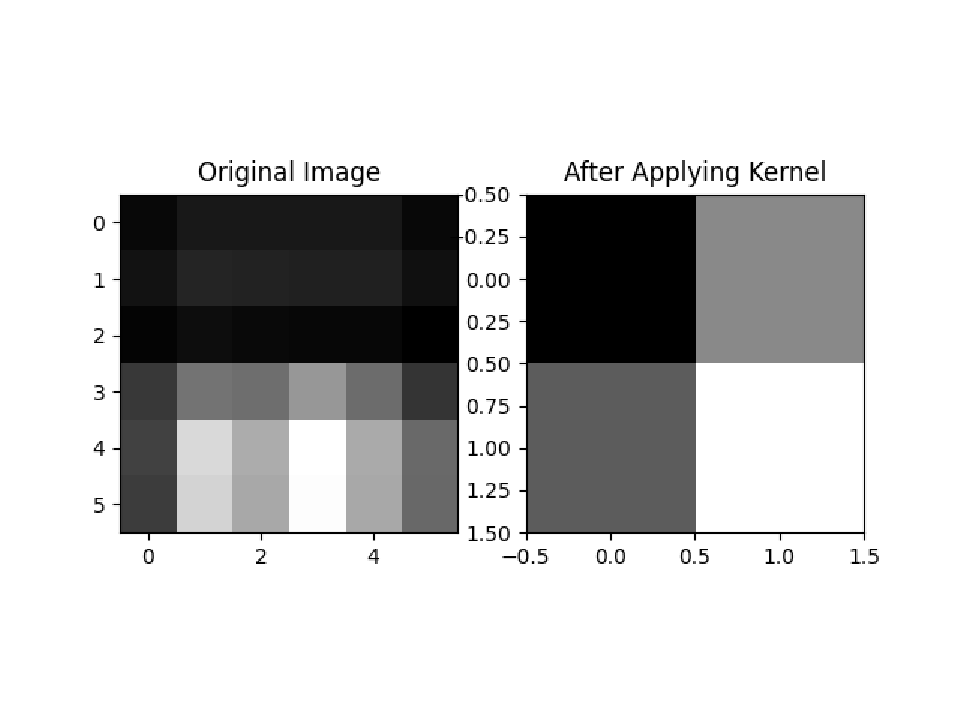
\includegraphics[width=.7\textwidth]{../Problem 11/kernel_F3.pdf}
		\caption{Before and After of the input image}
		\label{fig:kernel3}
	\end{figure}
	\vspace{3mm}
		
\end{itemize}
\vspace{5mm}






